\sectionquestion{Q-Learning and Deep RL}

\begin{parts}

\part Consider the following simple car environment with a perfectly flat road and a cliff on the right. The state $s = (p,v)$ consists of the position $p \in \{1,2,\ldots,10\}$ and velocity $v \in \{1,2,\ldots,10\}$, i.e. both $p$ and $v$ are discrete. The car only has 2 possible actions $a$ at each state: accelerate to the right, or do nothing (which causes the car to slow down). 
Neural wants to learn a policy for driving the car to the flag as fast as possible, but without driving off the cliff. 
%The reward function $R(s,a,s')=+1000$ if $s'$ has zero velocity and car overlaps the flag, $R(s,a,s')=-1000$ if $s'$ is beyond the edge of the cliff, $R(s,a,s')=0$ otherwise.


\begin{center}
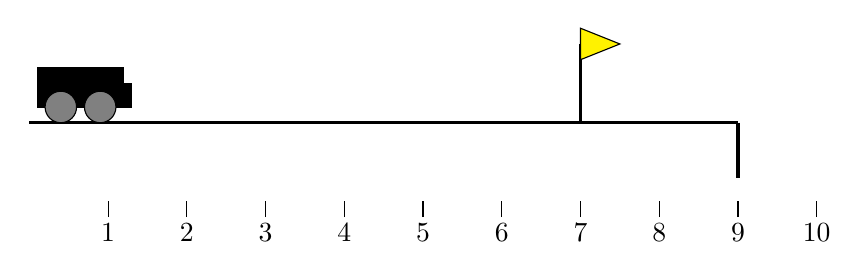
\begin{tikzpicture}

% Ground
\draw[very thick] (0,0) -- (9,0);

% Tick marks and labels
\foreach \x in {1,...,10} {
  \draw (\x,-1.2) -- (\x,-1);
  \node at (\x,-1.4) {\x};
}

% Cliff
\draw[very thick] (9,0) -- (9,-0.7);

% Flag pole
\draw[thick] (7,0) -- (7,1);

% Flag
\draw[fill=yellow] (7,0.8) -- (7.5,1) -- (7,1.2) -- cycle;

% Car body
\draw[fill=black] (0.1,0.2) rectangle (1.2,0.7);
\draw[fill=black] (0.1,0.2) rectangle (1.3,0.5);

% Car wheels
\draw[fill=gray] (0.4,0.2) circle (0.2cm);
\draw[fill=gray] (0.9,0.2) circle (0.2cm);

\end{tikzpicture}
\end{center}

Assume that $\gamma \in [0, 1)$, 
all rewards are bounded, 
the Q-values are initialized to 0, and $\alpha_t = \frac{1}{t+1}$. Transitions are deterministic.

\begin{subparts}

\subpart[2] \textbf{Short Answer:}  Neural uses tabular Q-learning to find $Q^*(s,a)$ for every state and action, and he runs 10,000 iterations. Neural claims that if he randomly chooses the initial state of the car at the start of each iteration and randomly selects each action, then he is guaranteed to converge to $Q^*(s,a)$ by the end of the training run. Is Neural's claim correct? Briefly justify your answer in 1-2 sentences.
    \fillwithlines{7em}
    \begin{soln} 
        Q is only guaranteed to converge to $Q^*$ if each (state, action) pair is also visited infinitely often. In this case, finite iterations and random state initialization makes it possible that some states are never visited at all.
    \end{soln}
    \begin{qauthor}
        Max, Identify the conditions under which the Q-learning algorithm will converge to the true value function
    \end{qauthor}

    % Sort of gives away the answer to the previous question.
    %
    % \subpart[2] \textbf{Short Answer:} Markov decides to run an infinite number of iterations, but at the start of each iteration, Markov always chooses an initial state with a position that is strictly to the left of the previous initial state. The position of the initial state in the first iteration is 10 (the flag). Is Markov guaranteed to converge to $Q^*(s,a)$? Briefly justify your answer in 1-2 sentences.\\ 
    % \fillwithlines{7em}
    % \begin{soln} 
    %     Yes, now every state is visited infinitely often, and the order in which states are visited doesn't matter in Q-learning.
    % \end{soln}
    % \begin{qauthor}
    %     Max, Identify the conditions under which the Q-learning algorithm will converge to the true value function
    % \end{qauthor}

\uplevel{For the questions below, the current state is $s$, the policy takes action $a$ and receives reward $r$, and transitions to state $s'$.}


\subpart[1] \textbf{Numerical answer:} For tabular $Q$-learning with this environment, how many table entries are there in the table $Q$?
    \begin{tcolorbox}[fit,height=1cm, width=4cm, blank, borderline={1pt}{-2pt}]
    %solution
    \end{tcolorbox}
    \begin{soln}
    200
    \end{soln}
    \begin{qauthor}
    Matt
    \end{qauthor}

\subpart[2] \textbf{Numerical answer:} Suppose the car is in state $s = (p=5, v=2)$ and the agent takes action `do nothing' so that we end in state $s'= (p=7, v=1)$ and receive reward $r=8$. Assume $\gamma$ is $0.5$. Suppose (for this problem only) that all $Q$ table entries were initialized to $4$. The Q-learning update rule would update one table entry. What is its new value?
    \begin{tcolorbox}[fit,height=1cm, width=4cm, blank, borderline={1pt}{-2pt}]
    %solution
    \end{tcolorbox}
    \begin{soln}
    $8 + 0.5 * 4 = 10$
    \end{soln}
    \begin{qauthor}
    Matt
    \end{qauthor}

\clearpage

\subpart[2] Consider applying two variants of Q-learning to this problem:
\begin{enumerate}
    \item[(A)] Apply the Q-learning update rule to a random past $(s, a, r, s')$ tuple and then randomly select the next action via $\epsilon$-greedy. Repeat.
    \item[(B)] Randomly select the next action via $\epsilon$-greedy and then immediately apply the Q-learning update rule to the current $(s, a, r, s')$. Repeat.
\end{enumerate}
\textbf{True or False:} In practice, variant (A) is unlikely to yield a better policy than variant (B) because environment is deterministic. \textbf{Briefly justify your answer.}
    \begin{checkboxes}
     \choice True 
     \choice False
    \end{checkboxes}
    \fillwithlines{8em}
    \begin{soln}
    False. Variant (A) is uniform experience reply which is likely to help because of the delayed/infrequent positive rewards.
    \end{soln}
    \begin{qauthor} Matt    \end{qauthor}

\subpart[2] \textbf{Select all that apply:} Now suppose the environment uses a stochastic transition distribution and stochastic rewards that simulate a Pittsburgh winter by allowing the car to randomly slip an extra position to the right at icy positions. Why would it be unwise to use the Q-learning update rule?
\begin{align*}
    Q(s,a) \gets r + \gamma \max_{a' \in \Ac} Q(s', a')
\end{align*}
    {%
    \checkboxchar{$\Box$} \checkedchar{$\blacksquare$} % change checkbox style locally
    \begin{checkboxes}
     \choice the current state $s$ might not be representative of the expected state $s$ at a given timestep in the trajectory
     \choice the action $a$ might not be representative of the most probable action under the $\epsilon$-greedy policy
     \choice the reward $r$ might not be representative of expected reward for the current $(s,a)$ pair
     \choice the next state $s'$ might not be representative of the most probable next state for the current $(s,a)$ pair
     \choice None of the above
    \end{checkboxes}
    }
    \begin{soln}
    C. and D. 
    \end{soln}
    \begin{qauthor}Matt
    \end{qauthor}
    
\end{subparts}


\part[1] \textbf{True or False:} If the state transition distribution and reward function are unknown, Q-learning cannot be used to learn a policy, but deep Q-learning can be applied.
    \begin{checkboxes}
     \choice True 
     \choice False
    \end{checkboxes}
    \begin{soln}
    False. Q learning and deep Q-learning can both be applied in this setting.
    \end{soln}
    \begin{qauthor}
    Matt
    \end{qauthor}


\part[1] \textbf{Fill in the blank by selecting one:} \textit{Deep Q-learning defines a neural network to approximate \underline{\hspace{8em}} which is helpful for very large \underline{\hspace{8em}} space(s)?}
    \begin{checkboxes}
     \choice $V(s)$  / state 
     \choice $V(s)$  / action 
     \choice $V(s)$  / state and action 
     \choice $Q(s,a)$ / state 
     \choice $Q(s,a)$ / action
     \choice $Q(s,a)$ / state and action
    \end{checkboxes}
    \begin{soln}
    $Q(s,a)$ / state
    
    TODO: rewrite this question since "action" and "state and action" are also perfectly valid answers
    \end{soln}
    \begin{qauthor}Matt
    \end{qauthor}

\end{parts}